\chapter{诊断算法透明性实验}

\section{实验设计}
我们通过在各大社交平台发布海报招募,如图\ref{fig:poster},以及使用问卷星的样本服务,招募了100位左右的用户。
\begin{figure}[htb]
    \centering
    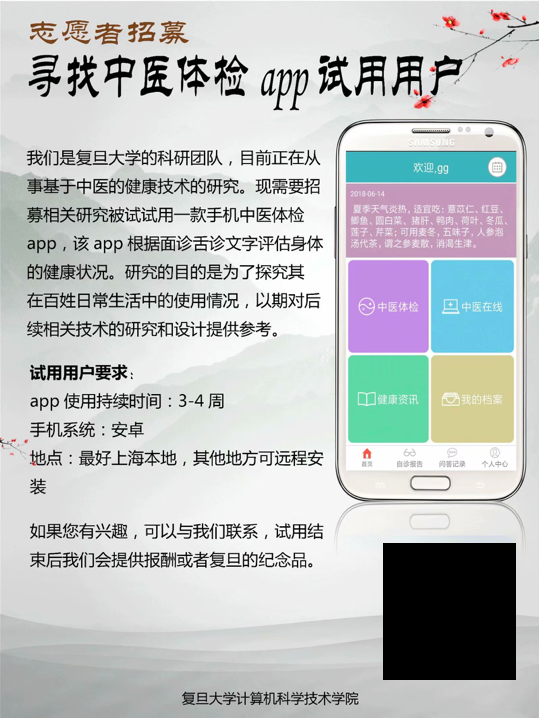
\includegraphics[height=12cm]{images/poster.png}
    \caption{招募海报}
    \label{fig:poster}
\end{figure}
\section{实验流程}
每个用户的实验流程如下:

1. 用户通过扫描二维码,或者通过我们给定的链接,进入问卷星调查问卷。

2. 完成调查问卷之后,自动进入云中医在线app。通过调用问卷星提供的企业用户接口, 同时把问卷星的问卷id传给云中医在线应用。

3. 在用户完成一次面诊之后,会在健康诊断页面下,看到一个跳转链接,可以选择填写用后问卷。



\section{实验数据获取}
因此,每个用户在参与实验之后,我们可以得到调查问卷的数据,云中医的使用日志,已经用后问卷的数据。三份数据可以通过问卷id和用户id链接起来,得到特征如表所示。

ID,性别,教育,工作,透明性,解释1,解释2,解释3,解释4,健康得分,信任、理解、前健康知识得分,后健康知识得分

\section{实验结果}
同时实验分析,我们可以得出,增加透明性可以提高用户对应中医知识的理解。



